\documentclass[12pt, a4paper, oneside]{book}
\usepackage[hidelinks]{hyperref}
\usepackage[slovak, english]{babel}
\usepackage{epsfig}
\usepackage{epstopdf}
\usepackage[chapter]{algorithm}
\usepackage{algorithmic}
\usepackage{listings}
\usepackage{amsmath}
\usepackage{amssymb}
\usepackage{graphicx}
\usepackage{multirow}
\usepackage{color}
\usepackage{url}
\usepackage[utf8]{inputenc}
\usepackage[T1]{fontenc}
\usepackage{setspace}
\usepackage{tabularx}
\usepackage{textcomp}
\usepackage{caption}
\usepackage[numbers]{natbib}

\selectlanguage{english}
\setstretch{1.5}
%\renewcommand\baselinestretch{1.5} % riadkovanie jeden a pol

\newcommand\mftitle{Deep Learning-based Human Pose Estimation from 3D Data}
\newcommand\mfthesistype{Master thesis}
\newcommand\mfauthor{Bc. Dana Škorvánková}
\newcommand\mfadvisor{RNDr. Martin Madaras, PhD.}
\newcommand\mfplacedate{Bratislava, 2020}
\newcommand\mfuniversity{COMENIUS UNIVERSITY BRATISLAVA}
\newcommand\mffaculty{FACULTY OF MATHEMATICS, PHYSICS AND INFORMATICS}
\newcommand{\sub}[1]{$_{\text{#1}}$}
\newcommand{\reference}[1]{č.~\ref{#1}}
\newcommand{\imageHeight}{180px}

\ifx\pdfoutput\undefined\relax\else\pdfinfo{ /Title (\mftitle) /Author (\mfauthor) /Creator (PDFLaTeX) } \fi

\begin{document}

\frontmatter

\thispagestyle{empty}

\noindent
\begin{minipage}{\textwidth}
\begin{center}
\textbf{\mfuniversity \\
\mffaculty}
\end{center}
\end{minipage}

\vfill
\begin{figure}[!hbt]
	\begin{center}
		
\includegraphics{images/logo_fmph}
		\label{img:logo}
	\end{center}
\end{figure}
\begin{center}
	\begin{minipage}{0.8\textwidth}
		\begin{center}\textbf{\Large\MakeUppercase{\mftitle}}\end{center}
		\smallskip
		\centerline{\mfthesistype}
	\end{minipage}
\end{center}
\vfill
2020 \hfill
\mfauthor
\eject 
% koniec obalu

\thispagestyle{empty}

\noindent
\begin{minipage}{\textwidth}
\begin{center}
\textbf{\mfuniversity \\
\mffaculty}
\end{center}
\end{minipage}

\vfill
\begin{figure}[!hbt]
\begin{center}

\includegraphics{images/logo_fmph_dark}
\label{img:logo_dark}
\end{center}
\end{figure}
\begin{center}
\begin{minipage}{0.8\textwidth}
\begin{center}\textbf{\Large\MakeUppercase{\mftitle}}\end{center}
\smallskip
\centerline{\mfthesistype}
\end{minipage}
\end{center}
\vfill
\begin{tabular}{l l}
%Registration number: & 40a99bd8-3cb6-4534-9330-c7fd9b5e5ca4 \\
Program of Study: & Applied Informatics\\
Field of Study: & 2511 Applied Informatics\\
Department: & Department of Applied Informatics\\
Supervisor: & \mfadvisor
\end{tabular}
\vfill
\noindent
\mfplacedate \hfill
\mfauthor
\eject 
% koniec titulneho listu

%\thispagestyle{empty}
%\includegraphics[width=\textwidth]{images/zadanie}
%\vfill
%\eject
% koniec zadania

\thispagestyle{empty}


\begin{figure}[H]
\begin{center}
\makebox[\textwidth]{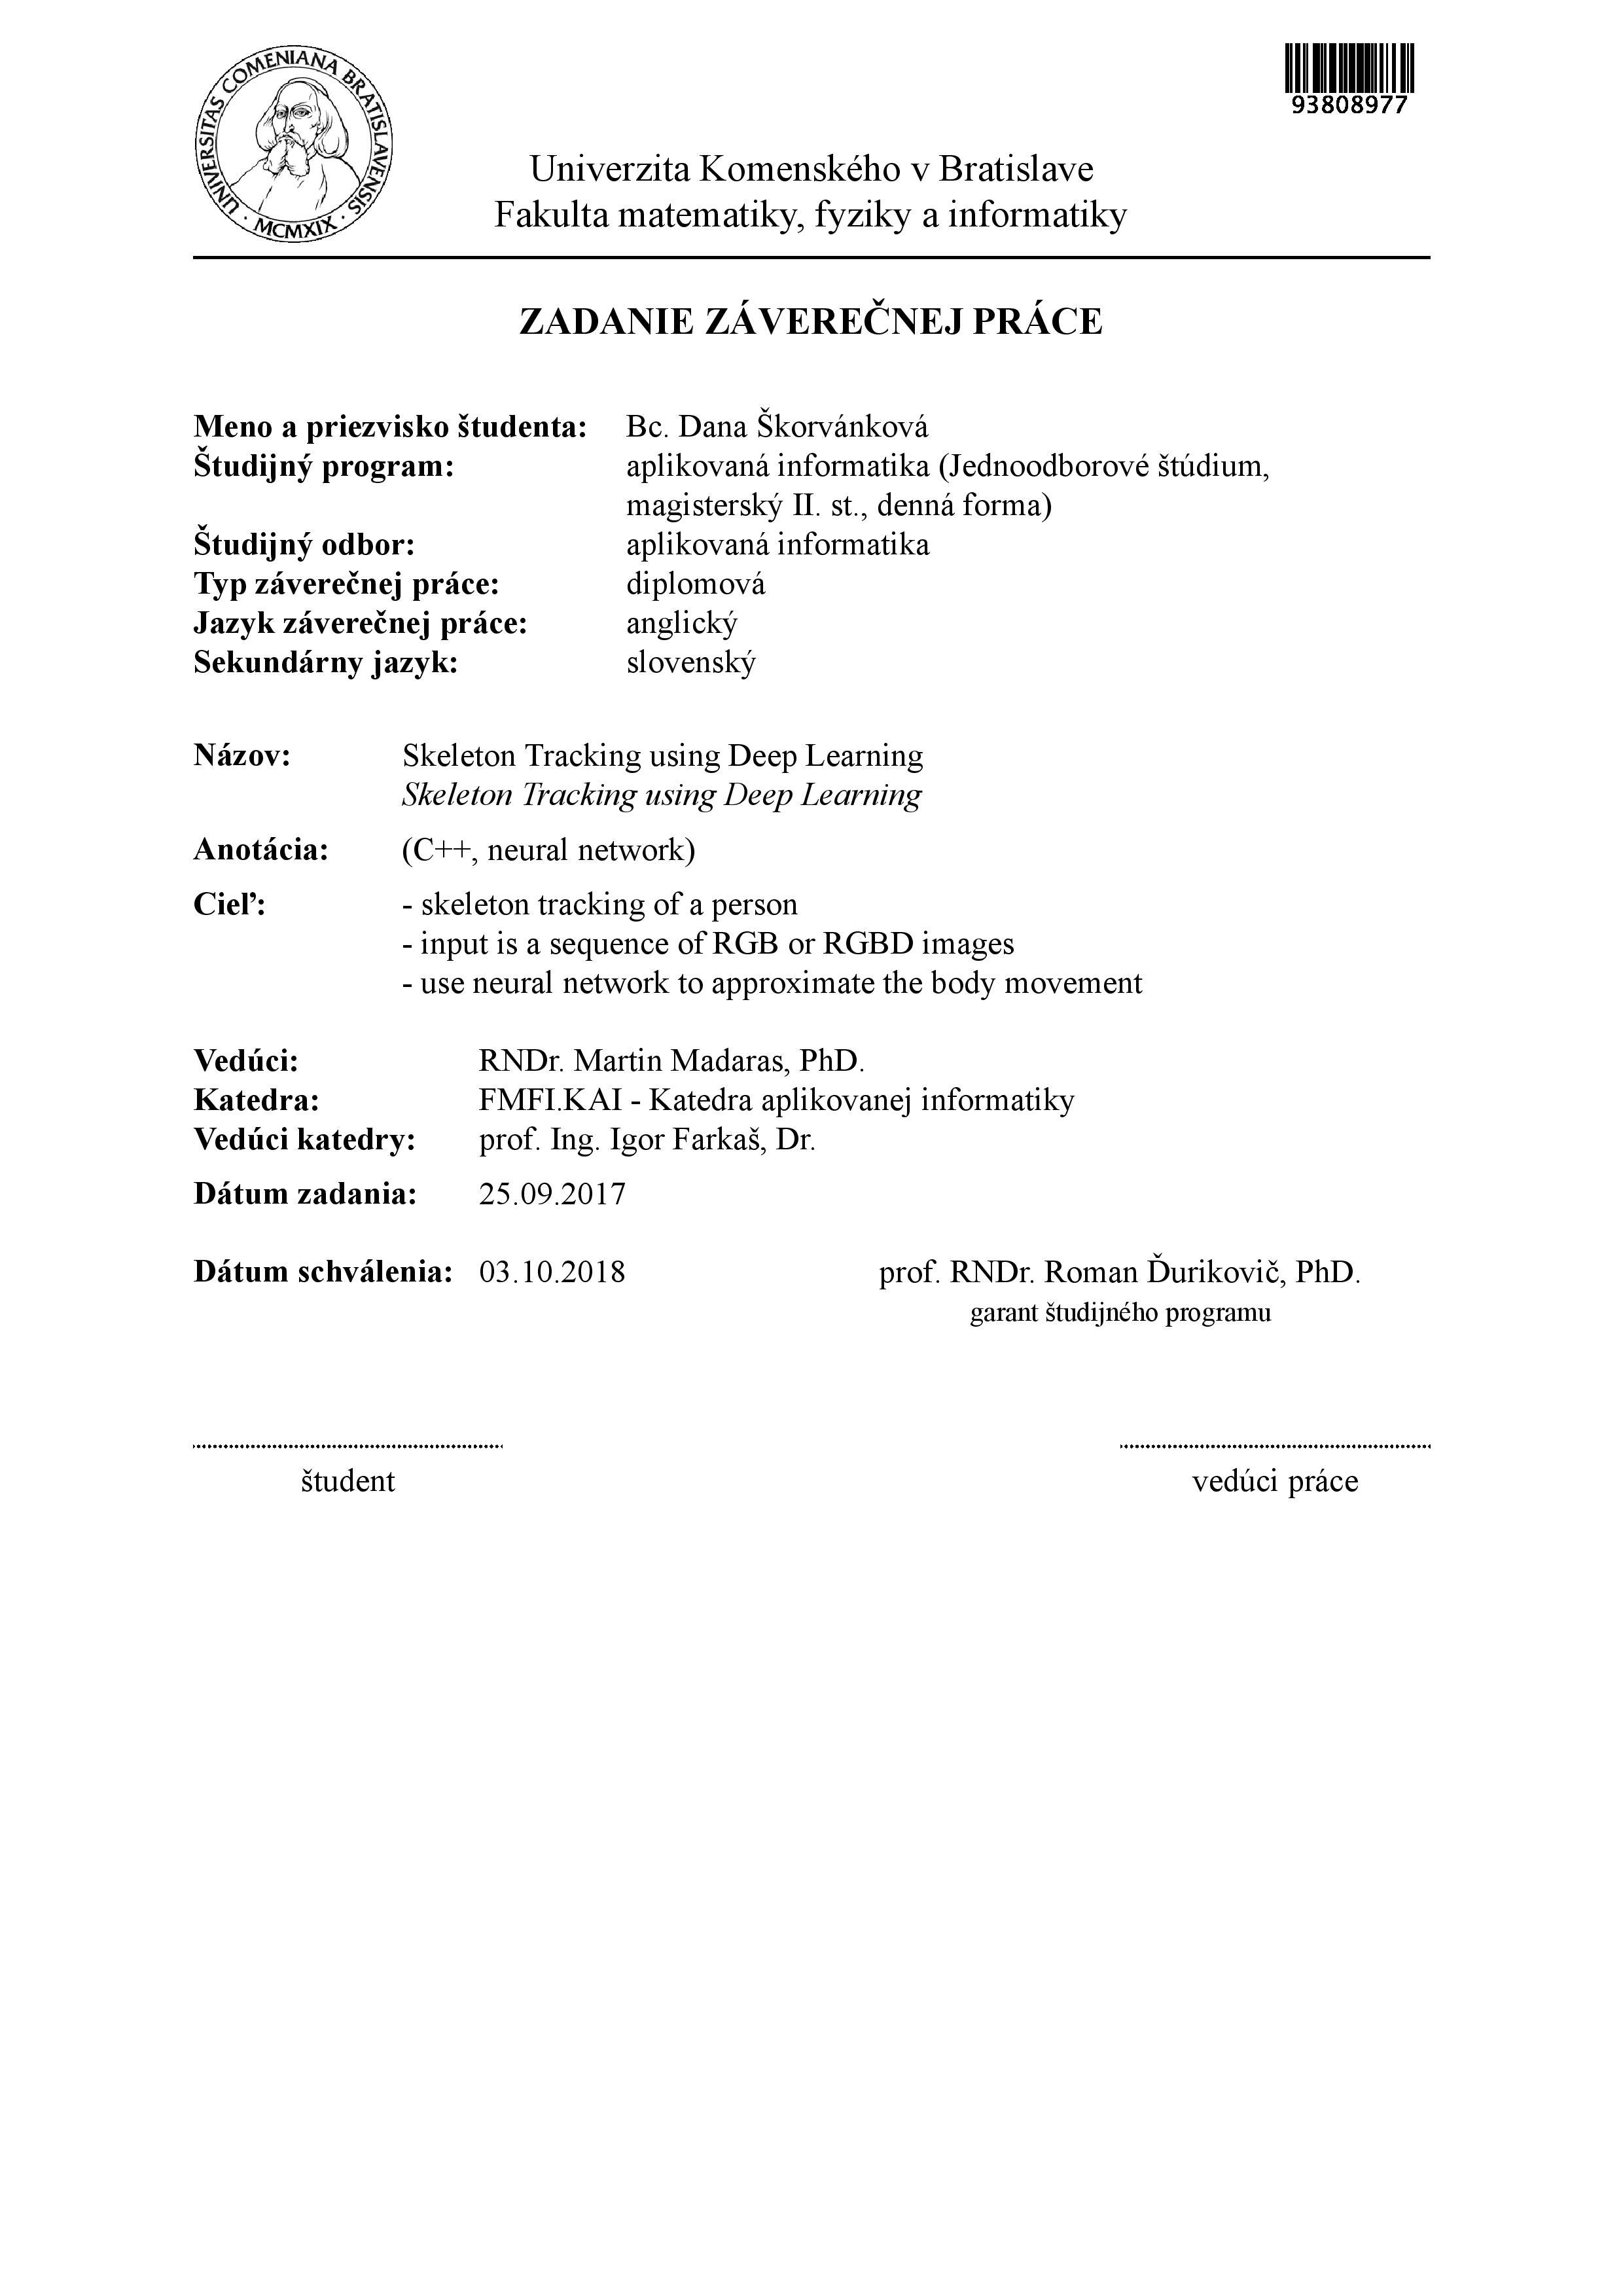
\includegraphics[width=\paperwidth]{images/master_thesis_assignment}} % TODO update
\label{img:zadanie}
\end{center}
\end{figure}

{~}\vspace{12cm}

\noindent
\begin{minipage}{0.25\textwidth}~\end{minipage}
\begin{minipage}{0.75\textwidth}
I hereby declare I wrote this thesis by myself, only with the help of
referenced literature, under the careful supervision of my thesis
supervisor.
\newline \newline
\end{minipage}
\vfill
~ \hfill {\hbox to 6cm{\dotfill}} \\
\mfplacedate \hfill \mfauthor
\vfill\eject 


\chapter*{Acknowledgement}\label{chap:thank_you}
I would like to thank my supervisor for his guidance and valuable feedback. Additionally, I would like to express my gratitude to
my family and close friends for all their patience and support.

\chapter*{Abstrakt}\label{chap:abstract_sk}
Cieľom tejto diplomovej práce je vyvinúť systém na 3D odhad pózy človeka, založený na neurónovej sieti, ktorý má na vstupe trojdimenzionálne dáta (vo forme mračna bodov alebo hĺbkovej mapy) a na výstupe vracia 3D koordináty vrcholov kostry. Máme v záujme prekonať obmedzenia spojené s vysokou nelinearitou priamej regresie 3D pózy z 2D obrazu využitím 3D vstupných dát, a zvýšiť tak presnosť odhadu. Naším zámerom je predstavenie nášho vlastného prístupu, ako aj implementácia niekoľkých existujúcich modelov, vynikajúcich svojimi výsledkami v rámci danej problematiky. Jednotlivé metódy následne evaluujeme na referenčných databázach, a porovnáme s doposiaľ najlepšími výsledkami dosiahnutými na uvedených dátach.

~\\
Kľúčové slová: 3D odhad pózy človeka, hlboké učenie, neurónové siete, mračná bodov
\vfill\eject 

\chapter*{Abstract}\label{chap:abstract_en}
The aim of our thesis is to develop a 3D human pose estimation pipeline based on neural network, which takes three-dimensional data (in a form of a point cloud or a depth map) as input and outputs the 3D skeletal joint coordinates. We intend to overcome the limitations associated with high non-linearity of direct regression from 2D image to 3D pose by inferring from 3D input data, and thus increase the estimation accuracy. Our goal is to introduce our own approach, in addition to implementing several well-performing models proposed in existing papers. Next, we aim to evaluate the methods on multiple benchmark datasets, and compare the results to the current state-of-the-art.

~\\
Keywords: 3D human pose estimation, deep learning, neural networks, point clouds
\vfill\eject 


\tableofcontents

\listoftables
\listoffigures

\mainmatter

\input 01intro.tex
\input 02motivation.tex
\input 03overview.tex
\input 04related_work.tex
\input 05proposal.tex
\input 06implementation.tex
\input 07results.tex
\input 08conclusion.tex

\backmatter

\nocite{*}
\bibliographystyle{authordate1}
\bibliography{references}



\end{document}